\chapter{Logistisk vækst af Lotka-Volterra's model}
I det tilfælde hvor byttedyrene, i Lotka-Volterra's model, har begrænset føde vil systemet bestå af differentialligninger med logistisk vækst. I det følgende vil logistisk vækst derfor blive forklaret.\\
\hfill \break

\section{Logistisk vækst}\label{lovaeg}
Hvis man forestiller sig at der ingen rovdyr er, da vil differentialligningen for byttedyr vokse eksponentielt, hvilket vil resultere i at antallet af byttedyrerne vil vokse uendeligt. Derfor tilføjes der en faktor for begrænset føde, så differentialligningen bliver på formen:

\begin{equation}\label{logvivp}
    \begin{cases}
    x'(t)&=ax(t)-bx(t)^2\\
    x(t_0)&=x_0
    \end{cases}
\end{equation}

Dette er en separabel differentialligning, og udfra dette kan vi tilføje en hjælpefunktion 
\begin{equation*}
    p(x)=ax-bx^2=ax\left(1-\frac{b}{a}x\right)
\end{equation*}
Ved faktorisering af $p(x)$ findes de værdier, hvor funktionen $x'(t)$ er lig $0$:
\begin{equation}
p(x)=0 \Leftrightarrow
    \begin{cases}
    &x_0 = 0,\\ 
    &x_0 = \frac{a}{b}
    \end{cases}
\end{equation}.

\begin{figure} [H]
    \centering
    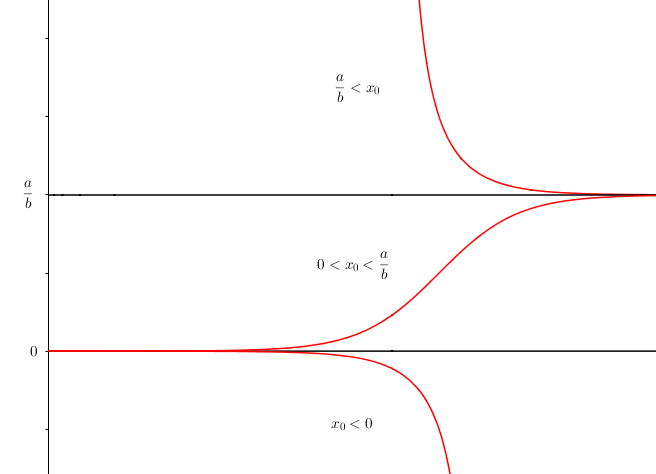
\includegraphics[scale=0.5]{Images/logi.png}
    \caption{Logistisk vækst}
    \label{logi}
\end{figure}

Ovenstånde figur illustrerer konklusionen af den kommende analyse for løsningskurver. Udfra den foregående faktorisering, vil der fremkomme fire mulige tilfælde for udseendet af løsningskurven til $t_0, x_0$:
\begin{enumerate}
    \item $x_0 = \frac{a}{b}, \ \textnormal{eller} \ x_0 = 0$ \\
    \item $0 < x_0 < \frac{a}{b}$\\
    \item $x_0 > \frac{a}{b}$ \\
    \item $x_0 < 0$ \\
\end{enumerate}
Tilfældene regnes nu igennem.

\subsubsection{Tilfælde 1}
Intuitivt ses det, at for tilfælde 1 vil tangenten være parallel med førsteaksen, og dermed vil løsningen gennem $(t_0, x_0)$ være konstant lig $x_0$. Grundet EES \citep{EES} er løsningen entydig. 
Altså har vi enten $x(t) \equiv \frac{a}{b}$ eller $x(t) \equiv 0$.\\
Vi giver her et argument for, at EES kan anvendes på det givne IVP \eqref{logvivp}.\\

\begin{enumerate}
    \item Funktionen $p(x)=ax-bx^2$ er defineret på hele $\mathbb{R}$ og afbilleder ind i $\mathbb{R}$. Dermed er $p \colon \mathbb{R}\times \mathbb{R}\to \mathbb{R}$.
    \item Hjælpefunktionen $p$ er kontinuert og differentiabel. Da eksisterer de partielle afledte, hvor $p'(x)=a-2bx$, som klart er kontinuert, da $p'(x)$ er et førstegradspolynomium.\\
    \item Det er trivielt opfyldt, da definitionsmængden er hele $\mathbb{R} \times \mathbb{R}$.\\ 
\end{enumerate}
Pér lemma \ref{th:LMD}, findes en løsning, $\phi(t)$, defineret på det maksimale definitionsinterval $]-\infty,\infty [$.

\subsubsection{Tilfælde 2}
Løsningskurven vil ligge i intervallet $\left] 0, \frac{a}{b} \right[$. Her vil den være være positiv og antage lokalt maksimum mellem $0$ og $\frac{a}{b}$.
Under følgende udregninger vil vi møde
\begin{equation*}
  \frac{1}{p(x)}=\frac{1}{ax-bx^2},
\end{equation*} 
hvor det er nødvendigt at finde dets stamfunktion. Her laves stambrøkdekomponering:

\begin{equation*}
    \frac{1}{ax(1-\frac{b}{a}x)}=\frac{A}{ax}+\frac{B}{1-\frac{b}{a}x}
\end{equation*}

For at finde værdierne, $A$ og $B$, sætter man på fælles brøkstreg:

\begin{equation*}
    \frac{A \left(1- \frac{b}{a}x \right)+Bax}{ax \left(1- \frac{b}{a}x \right)} =\frac{A + x \left( Ba-A \frac{b}{a} \right)}{ax \left(1-\frac{b}{a}x \right)}.
\end{equation*}

Udfra:
\begin{equation*}
\frac{1\cdot x^0+0\cdot x^1}{ax(1-\frac{b}{a}x)}
\end{equation*}

ses det, at $A=1$, og dermed er 
\begin{equation*}
    Ba - A \frac{b}{a} = 0 \Rightarrow B = \frac{1}{a} \cdot \frac{b}{a}.   
\end{equation*}

Da er 
\begin{align*}
    \frac{1}{p(x)} &= \frac{1}{ax}+\frac{\left( \frac{1}{a} \cdot \frac{b}{a} \right)}{1-\frac{b}{a}x} \\
    &= \frac{1}{ax \left( 1-\frac{b}{a}x \right)}
\end{align*}

Udfra foregående stambrøkskomponering kan vi udregne stamfunktionen, $H(x)$, til $\frac{1}{p(x)}$, jævnfør sætning \ref{th:LSD}:

\begin{align*}
    \int \frac{1}{ax}+\frac{ \frac{1}{a} \frac{b}{a}}{1-\frac{b}{a}x}dx
    &=\frac{1}{a}\ln|x|+\frac{\frac{1}{a}\frac{b}{a}}{-\frac{b}{a}}\ln \left|1-\frac{b}{a}x\right|\\
    &=\frac{1}{a}\ \ln|x|-\frac{1}{a}\ln \left|1-\frac{b}{a}x\right|
\end{align*}

Ved separation af $x'(t)$ i \eqref{logvivp} fås:
\begin{equation*}
    \frac{1}{(ax(t)-bx(t)^2)} x'(t)= 1   
\end{equation*}

Vi integrerer fra $t_0$ til $t$:
\begin{align*}
    \int^t_{t_0} \frac{1}{(ax(s)-bx(s)^2)} x'(s)ds&=\int^{t}_{t_0}1\ ds\\
    \left[ \frac{1}{a} \ln \left| \frac{x(s)}{1-\frac{b}{a}x(s)} \right| \right]^t_{t_0}&=[s]^t_{t_0}\\
    \frac{1}{a}\ln \left|\frac{x(t)}{1-\frac{b}{a}x(t)} \right|-\frac{1}{a}\ln \left| \frac{
    x_0}{1-\frac{b}{a}x_0} \right|&=t-t_0\\
    \ln \left| \frac{x(t)}{1-\frac{b}{a}x(t)}\right|-\ln \left|\frac{x_0}{1-\frac{b}{a}x_0}\right| &=a(t-t_0).
\end{align*}

Nu udredes, hvad $x(t)$ er, ved brug af logaritme regnereglerne:

\begin{equation*}
    \ln \left| \frac{x(t)}{x_0} \cdot \frac{1-\frac{b}{a}x_0}{1-\frac{b}{a}x(t)} \right| = a(t-t_0)
\end{equation*}

\begin{equation}\label{nur}
    \left|\frac{x(t)}{x_0}\right| \cdot \left| \frac{1-\frac{b}{a}x_0}{1-\frac{b}{a}x(t)} \right| 
    = e^{a(t-t_0)}
\end{equation}

For at fjerne de numeriske tegn ses der på, hvilken værdi de to brøker vil antage. Den første brøk vil blive positiv, da $\frac{a}{b}>x_0>0$, hvormed $x(t)>0$. Ses der på den anden brøk, vil også denne blive positiv, da $\frac{b}{a}x_0<\frac{b}{a}\frac{a}{b}=1$. \\
\hfill 
Da fjernes de numeriske tegn, og der isoleres for $x(t)$:

$$x(t) = \frac{x_0}{1 - \frac{b}{a}x_0} \left(1- \frac{b}{a}x(t) \right)e^{a(t-t_0)}$$

Nu sættes $K = \frac{x_0}{1 - \frac{b}{a}x_0}$:

\begin{align*}
x(t) &= K e^{(a(t-t_0))}-K \frac{b}{a}x(t) e^{a(t-t_0)} \\
\left(1+K \frac{b}{a} e^{a(t-t_0)}\right)x(t) &=K e^{a(t-t_0)} \\
x(t) &=\frac{K e^{a(t-t_0)}}{1+K \frac{b}{a} e^{a(t-t_0)}} = \frac{K e^{a(t-t_0)}}{K e^{a(t-t_0)}}\frac{1}{\frac{b}{a}+\frac{1}{Ke^{a(t-t_0)}}} \\
&= \frac{1}{\frac{b}{a}+(Ke^{a(t-t_0)})^{-1}} = \frac{1}{\frac{b}{a}+K^{-1}e^{-a(t-t_0)}} \\
&=\frac{1}{\frac{b}{a}+ \left( \frac{1-\frac{b}{a}x_0}{x_0} \right)e^{-a(t-t_0)}} \\
&=\frac{x_0}{ \left(1-\frac{b}{a}x_0 \right)e^{-a(t-t_0)}+ \frac{b}{a}x_0 }
\end{align*}

Da er $x(t)$ en løsning, som antager værdier i intervallet, $]0, \frac{a}{b}[.$

\subsubsection{Tilfælde 3}
Løsningskurven for dette tilfælde vil ligge i $\left] \frac{a}{b}, +\infty \right[$ og vil dermed være positiv.\\
\hfill \break
Dette tilfælde, samt tilfælde 4, vil følge en analog proces op til og med integrationen i \eqref{nur}.\\
\hfill \break

Det ønskes igen at fjerne de numeriske tegn. Det er givet, at $x_0 > \frac{a}{b}$, hvormed $x(t) > \frac{a}{b}$, og pér EES vil den første brøk være positiv. Den anden brøk vil også blive positiv, da $1-\frac{b}{a}x_0$ kun kan antage en negativ værdi, da $\frac{b}{a}x_0>1$, og det samme gælder for nævneren. Her kan vi isolere $x(t)$, ved samme fremgangsmåde som i tilfælde 2, og her vil man komme frem til samme $x(t)$:

\begin{equation}\label{logiloe1}
    x(t)= \frac{x_0}{ \left( \left(1- \frac{b}{a}x_0 \right)e^{-a(t-t_0)}+ \frac{b}{a}x_0 \right)}.
\end{equation}

Grundet, at $x_0>\frac{a}{b}$, kan nævneren i \eqref{logiloe1} antage værdien $0$. Det kan den idet, at $(1-\frac{b}{a}x_0)e^{-a(t-t_0)}<0$, og $\frac{b}{a}x_0>0$. Da findes der et $t_1$, hvor 

$$ \left(1- \frac{b}{a}x_0 \right)e^{-a(t_1-t_0)}+ \frac{b}{a}x_0 =0$$

Dette findes ved at isolere $t_1$ i ligningen. 

\begin{align*}
    e^{-a(t_1-t_0)}&=\frac{\frac{b}{a}x_0}{\left( \frac{b}{a}x_0 - 1 \right)}\\
    -a(t_1-t_0)&= \ln \frac{\frac{b}{a}x_0}{\left( \frac{b}{a}x_0 - 1 \right)}\\
    t_1&=t_0-\frac{1}{a}\ln\frac{\frac{b}{a}x_0}{\left(\frac{b}{a}x_0 - 1 \right)}
\end{align*}

Nu har vi fundet et udtryk for det $t_1$, hvor nævneren er $0$. For $x_0>\frac{a}{b}$, da er $x(t)$ defineret på $t>t_1$, fordi $x(t)$ divergerer mod $\infty^+$ for alle $t>t_1$. For alle $t<t_1$ vil $x(t)$ konvergere mod en given værdi, hvilket vil medføre et diskontinuitets hop. Det siges derfor, at der findes en lodret asymptote med ligningen,

\begin{equation*}
    t_1=t_0-\frac{1}{a}\ln\frac{\frac{b}{a}x_0}{\left(\frac{b}{a}x_0 - 1 \right)}
\end{equation*}


\subsubsection{Tilfælde 4}
Løsningskurven for dette tilfælde ligger i intervallet, $\left]- \infty , 0 \right[$, og vil dermed være negativ.\\
\hfill \break
For at fjerne de numeriske tegn kigger vi på funktionsværdien af $x$. Eftersom $x_0<0$, så er $x(t)<0$, dermed vil den første brøk blive positiv. Den anden brøk vil også blive positiv, da $1-\frac{b}{a}x_0$ kun kan antage en positiv værdi, da $-\frac{b}{a}x_0>0$, og det samme gælder for nævneren. Her kan vi isolere $x(t)$, ved samme fremgangsmåde som i tilfælde 2, og her vil man komme frem til samme $x(t)$:

\begin{equation}\label{logiloe2}
    x(t)= \frac{x_0}{ \left( \left(1- \frac{b}{a}x_0 \right)e^{-a(t-t_0)}+ \frac{b}{a}x_0 \right)}.
\end{equation}

Ligesom i tilfælde 3 kan nævneren i \eqref{logiloe2} antage værdien $0$. Her kigger vi på $x_0<0$, hvor $x(t)$ er defineret for $t<t_1$. Det er det samme som i tilfælde 3 bortset fra, at her vil $x(t)$ divergere mod $-\infty$ for alle $t<t_1$. 
\\ \hfill \break
Som en afsluttende bemærkning kan det nævnes at den ovenstående løsning i \ref{logiloe1} også er en løsning til differentialligningen:
\begin{equation}
    x'(t)=-ax(t)-bx(t)^2
\end{equation}
hvor konstanten $a$ i udtrykket for $x(t)$ blot er negativ. 
\section{Logistisk vækst af Lotka-Volterra's model}\label{lovaelovo}

Som sagt tilføjer vi en begrænset fødemængde til funktionen for byttedyrpopulationens vækst i Lotka-Volterra's model. Deruder over tilføjer vi også en kapacitetsbegrænsning til funktionen for rovdyrspopulationens vækst, hvilket giver et system på følgende form:

\begin{equation}\label{lovaeIVP}
\begin{aligned}
    b'(t) &=Ab(t)-Br(t)b(t)-Eb(t)^2\\
    r'(t) &=Db(t)r(t)-Cr(t)-Fr(t)^2,
\end{aligned}   
\end{equation}
med begyndelsesværdibetingelserne
\begin{equation}\label{IVPLovae}
    \begin{cases}
    b(t_0)&=b_0 \ , \ b_0\geq 0\\
    r(t_0)&=r_0 \ , \ r_0\geq 0
    \end{cases}
\end{equation}

Vi vil her igen indføre de to hjælpefunktioner $j$ og $l$.

\begin{equation}\label{hf1}
    j(b,r)=Ab-Brb-Eb^2
\end{equation}
\begin{equation}\label{hf2}
    l(b,r)=Dbr-Cr-Fr^2
\end{equation}
\hfill \break

Det vises nu, at modellen med logistisk vækst opfylder betingelserne i EESFS.

\begin{lemma}{Anvendelse af EESFS på logistisk vækst af Lotka-Volterra's model}{}
EESFS kan anvendes på logistisk vækst af Lotka-Volterra's model, som vist i systemet \eqref{lovaeIVP}, med begyndelsesværdibetingelserne \eqref{IVPLovae}.
\end{lemma}

\begin{proof}\\
    Vi tjekker, at de tre betingelser i EESFS er opfyldt.
    \hfill \break
    \begin{enumerate}
        \item Vektorfunktionen, $\vec{f}(\vec{b},\vec{r}) = (j(b,r),l(b,r))$, er defineret og kontinuert på hele $\mathbb{R}^3$, da $t$ ikke indgår eksplicit, og både $j$ og $l$ er definerede på hele $\mathbb{R}^2$. Vi har altså, at $\vec{f}\colon \mathbb{R}^3\to\mathbb{R}^2$.
        \item De partielle afledede eksisterer og er givet ved:
        \begin{equation*}
        \frac{\partial\vec{f}}{\partial \vec{y}}=
         \begin{bmatrix}
        \frac{\partial j}{\partial b} & \frac{\partial j}{\partial r}\vspace{1mm}\\
        \frac{\partial l}{\partial b} & \frac{\partial l}{\partial r}
        \end{bmatrix}
        =
        \begin{bmatrix}
        A-Br-2Eb & -Bb\\
        Dr & Db-C-2Fr
        \end{bmatrix}
        \end{equation*}
        Det ses, at alle de partielle afledede er førstegradspolynomier eller en sum af førstegradspolynomier, og dermed er de  $\frac{\partial\vec{f}}{\partial \vec{y}}$ kontinuerte. 
        \item Kravet til begyndelsesbetingelserne er trivielt opfyldt, da $\vec{f}$ er defineret på hele $\mathbb{R}^3$.
    \end{enumerate}
\end{proof}

For at finde nulklinerne for de to hjælpefunktioner $j$ og $l$, skal vi først omskrive vores funktioner, så vi kan anvende nulreglen: 

\begin{equation}\label{nulkliner1}
\begin{aligned}
    j(b,r)&=Ab - Brb - Eb^2     &   l(b,r)&=Dbr-Cr-Fr^2\\
    &=b(A - Br - Eb)     &   &=r(Db-C-Fr)\\
\end{aligned}    
\end{equation}
    Da er $j$-nulklinen givet ved $r$-aksen og linjen $r=\frac{A}{B}-\frac{E}{B}b$, og  $l$-nulklinen er givet ved $b$-aksen og linjen $b=\frac{C}{D}+\frac{F}{D}r$.\\ 

Systemets ligevægtspunkter er placeret, der hvor nulklinerne skærer hinanden, dermed sættes $j$-nulklinen og $l$-nulklinen lig hinanden, hvor der optræder fire  løsninger: 

\begin{align*}
    (b^*_1,r^*_1)&= (0,0), & (b^*_2,r^*_2)&= \left(0,-\frac{C}{F}\right), & (b^*_3,r^*_3)&= \left(\frac{A}{E},0\right), & (b^*_4,r^*_4)&= \left(\frac{AF+BC}{EF+BD},\frac{AD-EC}{EF+BD}\right)
\end{align*}
\hfill \break
Vi ønsker nu at betragte løsningskurvernes opførsel for startpunkter i første kvadrant. Det følgende er baseret på \citep[s. 257-259]{Svensk}.\hfill \break \\
Vi antager nu, at $EC>AD$ i dette tilfælde vil ligevægtspunktet $\left(\frac{AF+BC}{EF+BD},\frac{AD-EC}{EF+BD}\right)$ ligge i 4. kvadrant. 
Vi vil i det følgende vise, at hvis $b_0>0$ og $r_0>0$, så vil løsningskurverne for systemet ligge i første kvadrant. Vi ønsker, som i kapitel 5, at konstruere en løsning, der ligger på $b$-aksen henholdsvis $r$-aksen.\\ 
\hfill \break
Først vil vi konstruere en løsning, der ligger på $b$-aksen. Lad derfor $b_0 \in \mathbb{R}$ og $t_0 \in \mathbb{R}$ være givet. Hvis $r(t)\equiv 0$, så får vi fra ligning \eqref{IVPLovae}, at $b'(t)=Ab(t)-Eb(t)^2$. Det er en ligning på samme form som ligning \eqref{logvivp}. Dermed ses det af afsnit \ref{lovaeg}, at $b(t)= \frac{b_0}{ \left(1- \frac{E}{A}b_0 \right)e^{-A(t-t_0)}+ \frac{E}{A}b_0}$ er en løsning, som går gennem $(b_0,0)$ til tiden $t_0$, hvis $b_0>\frac{A}{E}$ eller $0<b_0<\frac{A}{E}$. Hvis $b_0=0$ eller $b_0=\frac{A}{E}$, så er $b(t)\equiv b_0$ en sådan løsning. I følge EESFS er disse løsninger entydige, hvorfor en løsningskurve ikke kan krydse den positive del af $b$-aksen.
\\ \hfill \break
 Lad nu $r_0\in \mathbb{R}$ og $t_0\in \mathbb{R}$ være givet. Hvis $b(t)\equiv 0$ så giver  ligning \eqref{IVPLovae}, at $r'(t)=-Cr(t)-Fr(t)^2$. Det ses, at $r(t)=\frac{r_0}{(1+\frac{F}{C}r_0)e^{C(t-t_0)}-\frac{F}{C}r_0}$ vil være en løsning med faseportræt på $r$-aksen, som går gennem $(0,r_0)$ til tiden $t_0$. Af samme grund som før, kan en vilkårlig løsning med begyndelsespunkt i 1. kvadrant ikke krydse $r$-aksen. Dermed kan en løsningskurve med begyndelsespunkt i 1. kvadrant ikke forlade denne.\\ 
 \hfill \break
Betragt nu nedenstående figur:

\begin{figure} [H]
    \centering
    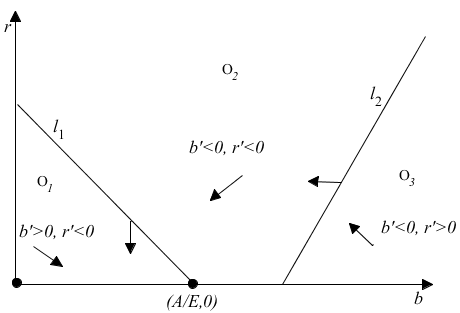
\includegraphics[scale=0.8]{Images/LoVae.png}
    \caption{Nullkliner \citep[s. 259]{Svensk}}
    \label{nulllovae}
\end{figure}

 Det ses, at nulklinerne deler det indre af 1. kvadrant op i 3 områder:
\begin{align*}
    O_1 &= \left\{(b,r) \in \mathbb{R}_+^2 \mid b \leq \frac{A}{E} , \ r \leq \frac{A}{B} - \frac{Eb}{B} \right\},\\
    O_2 &= \left\{(b,r) \in \mathbb{R}_+^2 \mid \frac{A}{E} - \frac{Br}{E} < b < \frac{C}{D} + \frac{Fr}{D} \right\},\\
    O_3 &= \left\{(b,r) \in \mathbb{R}_+^2 \mid b \geq \frac{C}{D} , \ r \leq -\frac{C}{F} + \frac{Db}{F}\right\}.
\end{align*}
Løsningskurverne igennem punkterne på $l_1$ vil have en tangent parallel med $r$-aksen, mens løsningskurverne igennem punkterne på $l_2$ vil have en tangent parallel med $b$-aksen.\\
I hvert af de tre områder, er $b'(t)$ og $r'(t)$ enten negativ eller positiv, som vist i figur \ref{nulllovae}. Vektorfeltets retning i hvert af de tre områder kan bestemmes på følgende måde. Vi indsætter konstanter i systemet \ref{lovaeIVP}, så uligheden $EC>AD$ er opfyldt. For eksempel:
\begin{equation*}
\begin{aligned}
    b'(t) &=\frac{1}{2}b(t)-\frac{1}{4}r(t)b(t)-\frac{1}{2}b(t)^2\\
    r'(t) &=\frac{1}{4}b(t)r(t)-\frac{1}{2}r(t)-\frac{1}{2}r(t)^2
\end{aligned}   
\end{equation*}
For at undersøge vektorfeltets retning i $O_1$ finder vi $b'(t)$ og $r'(t)$ i et punkt, som ligger i dette område. Dette punkt kunne for eksempel være $(1/4,1/4)$, og vi får: $b'(t)=\frac{5}{64}$ og $r'(t)=-\frac{9}{64}$. På samme måde findes vektorfeltets retning i de andre områder.\\ 
\hfill \break
De følgende argumenter er taget fra \citep[s. 258-259]{Svensk}. Lad os nu betragte løsningskurvernes opførsel i område $O_1$. På $l_1$ er $b'(t)=0$ og $r'(t)<0$, løsningskurverne vil derfor bevæge sig ind i det indre af $O_1$, hvor $b'(t)>0$ og $r'(t)<0$, og $b(t)$ er dermed en strengt voksende funktion, mens $r(t)$ er en strengt aftagende funktion i det indre af $O_1$. Da $b(t) \leq \frac{A}{E}$ er $b(t)$ altså opadtil begrænset i $O_1$ hvilket medfører, at der eksisterer et $\tilde{b} \geq 0$, så $\lim_{t \to \infty}b(t)=\tilde{b}$. I $O_1$ er $r(t)> 0$ og dermed nedadtil begrænset, hvilket medfører at der eksisterer et $\tilde{r} \geq 0$, så $\lim_{t \to \infty} r(t) = \tilde{r}$. 
\\  Løsningskurverne konvergerer altså mod et punkt, $(\tilde{b},\tilde{r})$, som må være et ligevægtspunkt for systemet ifølge følgende lemma:\\
\begin{lemma}{Grænseværdi for løsning \citep[s. 253]{Svensk}}{}
Lad $\vec{y}(t)$ være en løsning til et IVP, og lad IVP'ets maksimale definitionsinterval være $]a_1,\infty[$. Lad $\vec{y}(t)\to \hat{y}\in A$ for $t\to \infty$, hvor $A$ er defineret som i definition \ref{LoesningODE}. Så er $\hat{y}$ et ligevægtspunkt.
\end{lemma}
\begin{proof}\\
Lad $y_j(t)$ være den $j'$te koordinat i $\vec{y}(t)$. Da $\vec{y}(t)$ er en løsning, er $y_j(t)$ differentiabel på det åbne interval, $]t,t+1[ \ \subseteq \ ]a_1,\infty[$. Så følger det af middelværdisætningen, at
$$y_j(t+1)-y_j(t)= y_j'(\tau)=f_j(y_1(\tau),y_2(\tau),\hdots,y_n(\tau)),$$
 for et $\tau\in \ ]t,t+1[$, hvor $f_j$ er defineret som i definition \ref{autonom}. Når $t\to \infty$, går venstresiden mod $\hat{y}_j-\hat{y}_j=0$, og højresiden går mod $f_j(\hat{y})$. Dermed har vi, at $f_j(\hat{y})=0$ for alle $j$, og derfor er $\vec{f}(\hat{y})=0.$
\end{proof}\\ 
\hfill \break
Løsningskurverne i $O_1$ konvergerer altså mod et ligevægtspunkt.
Da $b(t)$ er strengt voksende i $O_1$, kan løsningskurverne ikke konvergere mod $(0,0)$, og den eneste mulighed er derfor $(\frac{A}{E},0)$.\\ 
\hfill \break
Vi betragter nu løsningskurverne med begyndelsespunkt i $O_2$. Det ses at $b'(t)< 0$ og $r'(t)<0$ i $O_2$, og både $b(t)$ og $r(t)$ er dermed aftagende funktioner. Grundet vektorfeltets retning kan en løsningskurve ikke bevæge sig ind i $O_3$, og den kan heller ikke skære akserne grundet EESFS. En løsningskurve, der forlader $O_2$, vil derfor gå ind i $O_1$, hvor vi ved, at den vil konvergere mod $(\frac{A}{E},0)$ for $t \to \infty$. Hvis løsningskurven forbliver i området $O_2$, ved vi, at $b(t)$ og $r(t)$ er aftagende og begrænsede funktioner. De har derfor en grænseværdi, og vi kan dermed anvende samme argumentation som før, for at vise at løsningskurverne konvergerer mod $(\frac{A}{E},0)$. \\ 
\hfill \break 
Til sidst betragtes løsningskurverne med begyndelsespunkt i $O_3$. På $l_2$ er $r'(t)=0$ og $b'(t)<0$. Derfor vil løsningskurverne bevæge sig ind i $O_2$. I det indre af $O_3$ er $r'(t)>0$ og $b'(t)<0$. Lad $(b_0,r_0)$ være et indre punkt i $O_3$ og lad $\Omega = \{(b,r) \in \mathbb{R}_+^2 | \frac{C}{D} \leq b \leq b_0, r \leq \frac{C}{F}+ \frac{Db}{F} \} $. Da $\Omega$ er en kompakt mængde, og $b'(t)$ er kontinuert, antager $b'(t)$ supremum på $\Omega$.
Sæt $S=\sup_{\Omega} b'(t)$, så er $b(t) \leq b_0 +tS$ i $\Omega$. Vi antager nu, at $b(t) \in \Omega  \ \forall t$. Da er $b(t) \geq \frac{C}{D}$. Men $\lim_{t \to \infty} b_0+tS= -\infty$, da $S<0$, hvilket medfører at $\lim_{t \to \infty} b(t)= -\infty$. Dette er en modstrid. Dermed eksisterer der et $t$, så $b(t)\leq \frac{C}{D}$. En løsningskurve, der starter i $O_3$, vil altså på et eller andet tidspunkt bevæge sig ind i $O_2$. Alle løsningskurver med et begyndelsespunkt i det indre af 1. kvadrant vil dermed konvergere mod $(\frac{A}{E},0)$.\\ 
\hfill \break 
I det ovenstående antog vi, at $a_2=\infty$ i det maksimale definitionsinterval $]a_1,a_2[$. Dette vil vi nu vise. Betragt nemlig figur \ref{nulllovae}. Det er klart, at $(b(t),r(t))\in [0,b_{max}]\times[0,y_{max}]$, som er en lukket og begrænset mængde. Antag nu, at $a_2\neq\infty$. Så er $(t,(b(t),r(t)))\in [0,a_2]\times[0,b_{max}]\times[0,y_{max}]$, som er en lukket og begrænset, og dermed kompakt, mængde. Derfor forlader den maksimale løsning denne mængde ifølge sætning \ref{forladkompakt}. Da $(b(t),r(t))\in [0,b_{max}]\times[0,y_{max}]$ for alle $t$, er den eneste mulighed, at $t$ forlader $[0,a_2]$. Det er en modstrid, og vi har altså at $a_2=\infty$. Det samme argument kan bruges for tilfældet, hvor $CE<AD$.
\\ \hfill \break
Vi antager nu, at $EC<AD$ i dette tilfælde vil ligevægtspunktet $(b_4^*,r_4^*)= \left(\frac{AF+BC}{EF+BD},\frac{AD-EC}{EF+BD}\right)$ ligge i 1. kvadrant. \\ \hfill \break
Som i tilfældet ovenfor kan vi bestemme vektorfeltets retning i de 4 områder; $O_1,O_2,O_3,O_4$, som er illustreret i figur (\ref{nulllovae2}).

\begin{figure} [H]
    \centering
    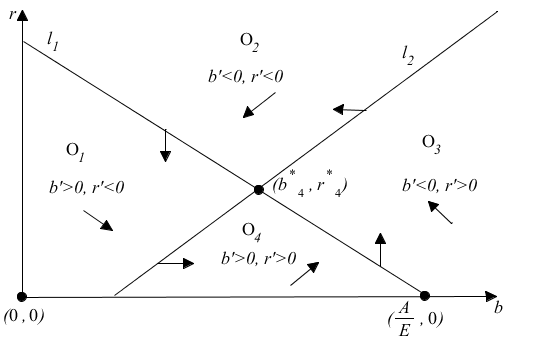
\includegraphics[scale=0.8]{Images/LoVae2.png}
    \caption{$(b_4^*,r_4^*)$ i 1. kvadrant.}
    \label{nulllovae2}
\end{figure}

Ved brug af de samme argumenter som i forrige tilfælde kan det vises at ligevægtspunktet $(b_4^*,r_4^*)$ er asymptotisk stabilt. \\ 
\hfill \break
Lad os først betragte løsningskurverne med begyndelsespunkt i $O_1$ og på $l_1$ for $r>r_4^*$. Hvis en sådan løsningskurve forlader området, $O_1$, vil den gå ind i $O_4$ på grund af vektorfeltets retning. Hvis den bliver i $O_1$, vil den konvergere mod $(b_4^*,r_4^*)$ med samme argument som før. Situationen er den samme i de andre områder. Enten konvergerer de mod $(b_4^*,r_4^*)$, eller de går ind i det næste område, jævnfør figur \ref{nulllovae2}. Dermed vil løsningskurverne med tiden bevæge sig ind mod ligevægtspunktet. Derfor er $(b_4^*,r_4^*)$ et asymptotisk stabilt ligevægtspunkt. 
\hfill \break

\section{Stabilitet af ligevægtspunkter i Lotka-Volterra med logistisk vækst}
Vi vender nu tilbage til systemets ligevægtspunkter og vil forsøge at beskrive dem ved hjælp af egenværdier.
Betragt Jacobi-matricen:
        \begin{equation}\label{jacobilovae}
        \textbf{J} =
        \frac{\partial\vec{f}}{\partial \vec{y}}=
         \begin{bmatrix}
        \frac{\partial j}{\partial b} & \frac{\partial j}{\partial r}\vspace{1mm}\\
        \frac{\partial l}{\partial b} & \frac{\partial l}{\partial r}
        \end{bmatrix}
        =
        \begin{bmatrix}
        A-Br-2Eb & -Bb\\
        Dr & Db-C-2Fr
        \end{bmatrix}
        \end{equation}
Hvis vi ser på ligevægtspunktet $(0,0)$ og indsætter dette i jacobi-matricen, fås:

        \[
        \textbf{J}_{\left(b^*_1,r^*_1 \right)} =
        \textbf{J}_{\left(0,0 \right)} =
        \begin{bmatrix}
        A & 0\\
        0 & -C
        \end{bmatrix}
        \]
Da er tilfældet det samme som for systemet uden logistisk vækst, og ligevægtspunktet er således et saddelpunkt. 
\hfill \break

Betragt nu Jacobi-matricen for $(b^*_2,r^*_2)$:
\begin{equation*}
    \textbf{J}_{\left(b^*_2,r^*_2 \right)} =
    \textbf{J}_{\left(0,-\frac{C}{F}\right)} =
        \begin{bmatrix}
        A + \frac{BC}{F} &  0\\
        -\frac{CD}{F} & C
        \end{bmatrix}
\end{equation*}
Vi indsætter denne matrix i vores ligning for at finde egenværdier:

$$
    \left(\textbf{J}_{\left(0,-\frac{C}{F}\right)}-\lambda I\right) =
        \begin{bmatrix}
        A + \frac{BC}{F} &  0\\
        -\frac{CD}{F} & C
        \end{bmatrix}-
    \begin{bmatrix}
    \lambda & 0\\
    0 & \lambda
    \end{bmatrix} =
        \begin{bmatrix}
        A + \frac{BC}{F} - \lambda &  0\\
        -\frac{CD}{F} & C - \lambda
        \end{bmatrix}
$$
Da findes $\det(\textbf{J}-\lambda I)$:

$$\left( A + \frac{BC}{F} - \lambda\right)(C - \lambda) = 0$$
Da er det klart, at egenværdierne for ligevægtspunktet $(0, -\frac{C}{F})$ er reelle og forskellige med samme fortegn, hvoraf det kan konkluderes, at ligevægtspunktet er en kilde og løsningskurverne vil bevæge sig væk fra ligevægtspunktet, hvorfor det er et ustabilt ligevægtspunkt, jævnfør \ref{tab:egenvardi}.
\hfill \break

Betragt nu Jacobi-matricen for $(b^*_3,r^*_3)$:
\begin{equation*}    
   \textbf{J}_{\left(b^*_3,r^*_3 \right)} =
    \textbf{J}_{\left(\frac{A}{E},0\right)} =
        \begin{bmatrix}
        -A &  \frac{AB}{E}\\
        0 & \frac{AD}{E}-C
        \end{bmatrix}
\end{equation*}
Vi indsætter denne matrix i vores ligning for at finde egenværdier:

$$
    \left(\textbf{J}_{\left(\frac{A}{E},0\right)}-\lambda I\right) =
        \begin{bmatrix}
        -A &  \frac{AB}{E}\\
        0 & \frac{AD}{E}-C
        \end{bmatrix}-
    \begin{bmatrix}
    \lambda & 0\\
    0 & \lambda
    \end{bmatrix} =
        \begin{bmatrix}
        -A - \lambda &  \frac{AB}{E}\\
        0 & \frac{AD}{E}-C-\lambda
        \end{bmatrix}
$$
Da findes $\det(\textbf{J}-\lambda I)$:

$$(-A - \lambda)\left(\frac{AD}{E}-C-\lambda\right) = 0$$

Egenværdierne er
\begin{align*}
    \lambda_1&=-A \\
    \lambda_2&=\frac{AD}{E}-C
\end{align*}

Det er nu klart, at egenværdierne for ligevægtspunktet $\left( \frac{A}{E} , 0 \right)$ er reelle. Egenværdierne for ligevægtspunktet vil enten være forskellige og med samme fortegn, eller forskellige med forskelligt fortegn alt efter hvilket led i $\lambda_2$, der er størst. 
I tilfældet, hvor $\frac{AD}{E} > C$, vil $\lambda_2 > 0$, og dermed er ligevægtspunktet et saddelpunkt og ustabilt. I tilfældet, hvor $\frac{AD}{E} < C$, vil $\lambda_2 < 0$, og dermed er ligevægtspunktet et dræn, hvormed løsningskurverne vil bevæge sig imod ligevægtspunktet, hvorfor det er asymptotisk stabilt, jævnfør tabel \ref{tab:egenvardi}. Dette stemmer overens med analysen i afsnit \ref{lovaelovo}. \hfill \break

%Jacobi-matricen for $(b^*_4,r^*_4)$ er en meget kompliceret beregning og vil derfor ikke blive undersøgt.% For simpelhedens skyld undersøges derfor tilfældet, hvor $F=0$. Derved er Jacobi-matricen:
% \begin{equation*}
%        \textbf{J} =
%        \begin{bmatrix}
%        A-Br-2Eb & -Bb\\
%        Dr & Db-C
%        \end{bmatrix}
%        \end{equation*}
%Ligevægtspunktet vil også ændres til $(b^*_4,r^*_4)=(\frac{BC}{BD}, \frac{AD-EC}{BD})$. Ved indsættelse i Jacobi-matricen fås derved:
%\begin{equation*}
%    \textbf{J}_{\left(b^*_4,r^*_4 \right)} =
%     \begin{bmatrix}
%        A-B\frac{AD-EC}{BD}-2E\frac{BC}{BD} &  -B\frac{BC}{BD}\\
%        D\frac{AD-EC}{BD} & D\frac{BC}{BD}-C
%        \end{bmatrix}
%    =\begin{bmatrix}
%        -\frac{EC}{D} & -\frac{BC}{D}\\
%        \frac{AD-CE}{B} & 0
%        \end{bmatrix}
%\end{equation*}
%Det karakteristiske polynomium til denne matrix er derved
%\begin{equation*}
%    \det(\textbf{J}_{\left(b^*_4,r^*_4 \right)}-\lambda I_4)= \lambda^2+\lambda\frac{EC}{D}+\frac{C(AD-CE)}{D}=0
%\end{equation*}
%   
%Diskriminanten dertil er
%\begin{align*}
%    &d=\left(\frac{EC}{D}\right)^2-4\left(AC-\frac{CE^2)}{D} \right)
%\end{align*}
% \hfill \break
%og egenværdierne er
%\begin{align*}
%   \lambda&=-\frac{EC}{2D} \pm \frac{1}{2}\sqrt{\left(\frac{EC}{D}\right)^2-4\left(AC-\frac{CE^2}{D} \right)}\\
%   &= -\frac{EC}{2D} \pm \sqrt{\left(\frac{EC}{2D}\right)^2-\left(AC-\frac{CE^2}{D} \right) } \\
%   &= -\frac{EC}{2D} \pm \sqrt{\left(\frac{EC}{2D}\right)^2-AC\cdot\left(\frac{EC}{D}\right)^2\cdot\frac{4D^2}{E^2C^2}-\frac{CE^2}{D}\cdot\left(\frac{EC}{D}\right)^2\cdot\frac{4D^2}{E^2C^2}}\\
%   &=\left(\frac{EC}{2D}\right)^2 \left(-1\pm \sqrt{1+\frac{4D}{E}-\frac{4AD^2}{E^2C}}\right)
%\end{align*}

%Dermed kan det fastslås, at egenværdierne er komplekst konjugerede værdier med negativ realdel, hvis
%\begin{align}
%    E<4D\left(\frac{AD}{EC}-1\right),
%\end{align}
%og dermed må ligevægtspunktet $(b^*_4,r^*_4)$ være asymptotisk stabilt for disse $E$, og løsningskurven vil bevæge sig i en spiral ind mod dette punkt.
%\hfill \break
%Dermed må det være muligt at finde en streng Lyapunov funktion i ligevægtspunktet.
%\hfill \break 

I det følgende antages det, at uligheden $AD > EC$ er opfyldt, og Jacobi-matricen for $(b^*_4,r^*_4)$ betragtes.
Først indser vi, at $(b^*_4,r^*_4)$ er et ligevægtspunkt, hvor $j$-nulklinen og $l$-nulklinen krydser. Da ligevægtspunktet ligger i det indre af 1. kvadrant, må der gælde, at $r > 0$ og $b > 0$, hvoraf $j$- og $l$-nulklinerne, pér \eqref{nulkliner1}, er givet ved:
\begin{align*}
    A - Br - Eb &=0\\
    Db -C -Fr &=0
\end{align*}
Da fås, jævnfør ligning \eqref{jacobilovae}:
 \begin{equation*}
    \textbf{J}_{(b_4^*, r_4^*)} = \textbf{J}_{(\frac{AF+BC}{EF+BD}, \frac{AD-EC}{EF+BD})} = \begin{bmatrix}
    -E\left( \frac{AF+BC}{EF+BD}\right) & -B\left( \frac{AF+BC}{EF+BD} \right) \\
    D \left(\frac{AD-EC}{EF+BD} \right) & -F \left( \frac{AD-EC}{EF+BD}\right)
        \end{bmatrix}.
\end{equation*}


For overskuelighedens skyld benyttes $(b_4^*,r_4^*)$ indledningsvist i det følgende. Først findes $\det(\textbf{J}_{(b_4^*,r_4^*)}-\lambda I)$:
\begin{align*}
   \det(\textbf{J}_{(b_4^*,r_4^*)}-\lambda I) &= \left( -Eb_4^* -\lambda \right) \left( -F r_4^*-\lambda\right)+ Dr_4^*Bb_4^* \\
   &=\lambda^2 + (Eb_4^* + F r_4^*)\lambda + (EF(b_4^*r_4^*) + DB(b_4^*r_4^*))
\end{align*}
Fra dette udledes, at $4(EF(b_4^*r_4^*) + DB(b_4^*r_4^*)) > ((Eb_4^* + F r_4^*)\lambda)^2$, hvis der skal eksistere komplekse rødder for den karakteristiske ligning, som også kan skrives som,
$$((ADF+AEF+BCE-CEF)\lambda)^2 < 4(A^2DF+ABCD-ACEF-BC^2E)$$






%\begin{align*}
%   \det(\textbf{J}_{(b_4^*,r_4^*)}-\lambda I) &= \left( -E\left( \frac{AF+BC}{EF+BD}\right)-\lambda \right) \left( -F \left( \frac{AD-EC}{EF+BD}\right)-\lambda\right)+ \frac{D(AD-CE)B(AF+BC)}{(BD+EF)^2} \\
%   &=\lambda^2 + \frac{(ADF+AEF+BCE-CEF)\lambda}{BD+EF}+\frac{A^2DF+ABCD-ACEF-BC^2E}{BD+EF}.
%\end{align*}
\textbf{Vi har ikke vist at rødderne til det karakteristiske polynomium er komplekse. I det følgende antager vi imidlertid, at det gælder.}
I den videre bearbejdelse af ligevægtspunktet, $\textbf{J}_{(b^*_4, r^*_4)}$, antages det, at det karakteristiske polynomium, som beskrevet ovenfor, har komplekse rødder. Der indføres nu følgende lemma, for at gøre analysen af egenværdier for $\textbf{J}_{(b^*_4, r^*_4)}$ mulig:
\begin{lemma}{Den komplekskonjugerede rodsætning}{egvdjacobi}
Hvis $\lambda^2 + a \lambda +b=0$, hvor $a, b \in \mathbb{R}$ har en kompleks rod, $\lambda_0$, så er $\bar{\lambda}_0$ også en rod.
\end{lemma}

\begin{proof}\\
Lad $\lambda_0 \in \mathbb{C}$ være en rod til $\lambda^2 +a \lambda +b = 0$, hvor $a, b \in \mathbb{R}$. Da fås ud fra $\lambda_0^2 +a \lambda_0 +b = 0$, at
$$(\bar{\lambda_0})^2 +a \bar{\lambda}_0 +b = \bar{0}=0,$$
hvormed $\bar{\lambda}_0$ også er en rod.
\end{proof}
\\ \hfill \break
\textbf{Bemærk:} Lemma \ref{th:egvdjacobi} fortæller, at når $\lambda_0 = \alpha + i \beta$ fås, så gælder følgende
\begin{align*}
    \lambda^2 +a\lambda +b &= (\lambda-(\alpha +i \beta))(\lambda - (\alpha - i \beta)) \\
    &= (\lambda - \alpha)^2 -(i \beta)^2 \\
    &= \lambda^2-2 \alpha \lambda + \alpha^2 + \beta^2.
\end{align*}
Hvormed
\begin{equation*}
\begin{cases}
    a &= -2 \alpha, \\
    b &= \alpha^2 + \beta^2.
\end{cases}
\end{equation*}
Dermed er det nok at kende fortegnet på $a$, for at bestemme fortegnet på realdelen af roden.\\ \hfill \break
Det ønskes kun at undersøge egenværdierne for ligevægtspunktet, når det eksisterer i det indre af 1. kvadrant, da løsningskurverne, i det tilfælde hvor ligevægtspunktet er i 4. kvadrant, vil ende i ligevægtspunktet $(b^*_3, r^*_3)$. Ligevægtpunktet, $(b^*_4, r^*_4)$, ligger i det indre af 1. kvadrant, når uligheden, $AD > CE$, er opfyldt. Ved brug af denne ulighed ses det, at
$$\frac{(ADF+AEF+BCE-CEF)}{BD+EF} > 0,$$
og dermed vil egenværdierne $\lambda_0$ og $\bar{\lambda}_0$ for
$\textbf{J}_{(b^*_4, r^*_4)}$ have negativ realdel. Derfor er ligevægtspunktet, $(b^*_4, r^*_4)$, et spiralpunkt.
\hfill \break

En anden metode der kan benyttes er en Lyapunov funktion. Følgende proposition undersøges. 
\begin{prop}{Eksistens af streng Lyapunov funktion i logistisk vækst af Lotka-volterra's model}{elovae}
$E_f(u, v) = \left( u-b^* \ln{\left( \frac{u+b^*}{b^*} \right)} \right) + \frac{B}{D} \left( v-r^* \ln{\left( \frac{v+r^*}{r^*} \right)} \right)$, hvor $u=b-b^*, v=r-r^*$, er en streng Lyapunov funktion til systemet \eqref{lovaeIVP}.
\end{prop}

\begin{proof}
Det efterprøves om Lyapunov funktionen er lig 0, ved ligevægtspunktet $(b_4^*,r_4^*)$
$$E(b^*, r^*) =  \left( 0-b^* \ln{(1)} \right) + \frac{B}{D} \left( 0-r^* \ln{(1)} \right)=0.$$
 
Det ses at, når $u=0=v$ er der tale om et ekstremumspunkt, da $\frac{\partial E}{\partial u}(0,0)=0$ og $\frac{\partial E}{\partial v} (0,0)=0$. Hesse matricen undersøges nu for $E$:. 
 \begin{align*}
     H&=\begin{bmatrix}
     \frac{ b^*}{(u+b^*)^2} & 0 \\
     0 & \frac{\frac{B}{D}\cdot r^*}{(v+r^*)^2}
     \end{bmatrix}\\
     \det (H)&= \frac{ b^*}{(u+b^*)^2} \cdot \frac{\frac{B}{D} r^*}{(v+r^*)^2} > 0 \ \text{for} \ b,r>0\\
     \textnormal{trace}(H)&= \frac{ b^*}{(u+b^*)^2} + \frac{\frac{B}{D} r^*}{(v+r^*)^2} > 0 \ \text{for} \ b,r>0\\
 \end{align*}
 
 Jævnfør sætning \ref{th:Hesse}, ligning \eqref{det10} og \eqref{trace} er punktet dermed lokalt minimum for $E$, og $E(u,v) > 0$ for $u \neq 0, v \neq 0$.
 \hfill \break
Det undersøges nu, om $E$ er streng Lyapunov funktion, $\dot{E}_f < 0$:
$$\dot{E}_f (b, r)=\frac{\partial E}{\partial u}j(b,r) + \frac{\partial E}{\partial v}l(b,r) =  \left( 1 - \frac{b^*}{u+b^*}\right) b (A-Eb-Br) + \frac{B}{D} \left( 1 - \frac{r^*}{v+r^*}\right) r (Db-Fr-C),$$
hvis $AD > EC \Rightarrow b^*, r^* > 0$, så er de skrå nulkliner
$$A-Eb^*-Br^* = 0$$
$$Db^*-Fr^*-C = 0.$$

Vi kan nu subtrahere 0 fra udtrykket: 
\begin{align*}
    A-Eb-Br &= A-Eb-Br-(A-Eb^*-Br^*) \\
    &=-E(b-b^*)-B(r-r^*) \\
    &=-Eu-Bv,
\end{align*}
og
\begin{align*}
    Db-Fr-C &= Db-Fr-C-(Db^*-Fr^*-C) \\
    &=D(b-b^*)-F(r-r^*) \\
    &=Du-Fv.
\end{align*}

Derfor
\begin{align*}
    \dot{E}_f(u, v) &= \left( u + b^* - \frac{b^*(u+b^*)}{u+b^*} (-Eu-Bv) \right) + \frac{B}{D} \left( v + r^* - \frac{r^*(v+r^*)}{v+r^*} (Du-Fv) \right) \\
    &= u(-Eu-Bv) + \frac{B}{D} v(Du-Fv) \\
    &= (-Eu^2-Bvu) + \frac{B}{D} (Duv-Fv^2) \\
    &= - Eu^2- \frac{B}{D}  Fv^2 -(\frac{B}{D} - B)uv
\end{align*}
Dette kan også skrives på matrix form:
\begin{align*} 
&= \dot{E}_f(u,v). \\
&= -  Eu^2- \frac{BFv^2}{D}-(\frac{B}{D} - B)uv \\
&= - \frac{1}{2} (2E u^2 + \frac{FB}{D} v^2 + 2 uv(B - \frac{B^2}{D})) \\
&= - \frac{1}{2} \begin{bmatrix}
2E u + v(B + B) & \frac{2EB}{D} v 
\end{bmatrix}
\begin{bmatrix}
u \\
v
\end{bmatrix}\\
&= - \frac{1}{2} \begin{bmatrix}
u & v
\end{bmatrix} 
\begin{bmatrix}
2E & 0 \\
0 & \frac{2FB}{D}
\end{bmatrix}
\begin{bmatrix}
u \\
v
\end{bmatrix} 
\end{align*}

Vi betegner nu $S:= \begin{bmatrix}
2E & 0\\
0 & \frac{2FB}{D}
\end{bmatrix}$. Vi ønsker nu at undersøge om $\vec{l}^T S \vec{l} > 0$. Altså undersøges om $S$ er positivt definit for en given vektor $\vec{l} \neq 0$.
Matricen $S$ er symmetrisk. For at være positivt definit skal egenværdierne for $S$ være positive. Dette betyder at determinanten og sporet skal være positive. 
Altså $$\det (S) > 0 \ \textnormal{og} \ \textnormal{trace} (S) > 0,$$ hvor $\textnormal{trace}(S)=\lambda_1 + \lambda_2$ og $\det(S)=\lambda_1\lambda_2$. Dermed: 
\begin{align*}
    \textnormal{trace(S)} &=2E + \frac{2FB}{D}> 0\\
    \det(S) &=\frac{4EFB}{D} >0 \\
\end{align*}

Dermed er $E(b,r)$ streng Lyapunov funktion i første kvadrant.

\end{proof}\\ \hfill \break